\documentclass[class=book, crop=false]{standalone}
\usepackage[utf8]{inputenc}
\usepackage[subpreambles=true]{standalone}
\usepackage{import}
\usepackage[ruled,vlined]{algorithm2e}

\usepackage{amsmath}
\usepackage{amssymb}
\usepackage[margin=1.2in]{geometry}
\usepackage[sorting = none,
            doi = true  %lesedato for url-adresse
            ]{biblatex} %none gir bibliografi i sitert rekkefølge
\addbibresource{reference.bib}
\usepackage{csquotes}
\usepackage{pgfplots}
\pgfplotsset{compat=1.15}


\begin{document}
%\chapter{Reinforcement learning}
\section{Intuitive introduction to reinforcement learning}
Reinforcement learning is an algorithm that learns through trial and error. The system consists of an agent that observes a state and responds to that by taking an action. Simply put, the agent will get a positive reward when it takes good actions and negative rewards for bad actions. When the agent takes a bad action, it will be less likely to chose that action again later. Similarly, when it gets a positive reward it will more likely chose a similar action given the same observed state. By letting the agent see many states and explore different actions, it can eventually learn a behaviour that harness a lot of positive rewards. 

Reinforcement algorithms are similar to how humans and animals learn. Imagine a dog seeing its owner holding a bag of treats. Obviously, the dog is keen on getting the treats, but is not sure what to do. The dog sees that the owner is putting his hand in front of its nose and yelling some command, but does not quit understand what to do. So it simply tries doing something. First, it might try to lean forward and smell the hand. Sadly, this does not result in any treat. Therefore, it continuous to try different actions, until it eventually happens to lift its front paw in the hand of the owner. At last, it receives a tasty treat from the owner. It has learned what action to take to get a treat. Next, the owner might rotate its arm in front of the dog. The dog might try to lift its front paw again, since that worked last time. Sadly, it does not get a reward this times. Therefore, it starts to explore new actions until it after some time tries to spin around. Again, it receives a treat. It has now learned that simply raising its front paw does not always result in a treat. It has to evaluate its observation before taking an action. 

The dog training is similar to the mechanisms in a reinforcement learning algorithm. The dog is the agent that tries to figure out what actions to do, while the owner is the reward system. The advantage of a reinforcement algorithm is that it does not need a physical reward, but is happy with a numerical reward. In addition, a computer can experiment much more quickly and efficient than a dog can. 

\section{Reinforcement learning and machine learning}
Algorithms in machine learning and artificial intelligence are often divided into either supervised or unsupervised learning. Supervised learning is an algorithm using input data and labelled output data (target). The algorithm tries to map the input to the target in a manner that generalises well to unseen input data. Examples of supervised learning are regression and classification algorithms. Algorithms using unsupervised learning attempt to find structure in unlabelled data. In other words, the goal is not to find a mapping between input and output as there is no output data. Examples of unsupervised learning are clustering and anomaly detection. The terms \textit{supervised} and \textit{unsupervised} do not describe well the mechanisms of reinforcement learning algorithms. A reinforcement learning agent learns from interaction with an environment and receiving rewards based the action it takes. The agent's goal is not to use labelled data in some sense or explicitly finding general structures in the data. As a result, reinforcement learning is considered to be a category of its own \cite{Sutton1998}. However, it should be noted that there are reinforcement algorithm that use supervised learning in the learning process. The relation between supervised, unsupervised and reinforcement learning is shown in figure \ref{fig:theory:supervised_vs_rl}


\begin{figure}[ht!]
    \center
    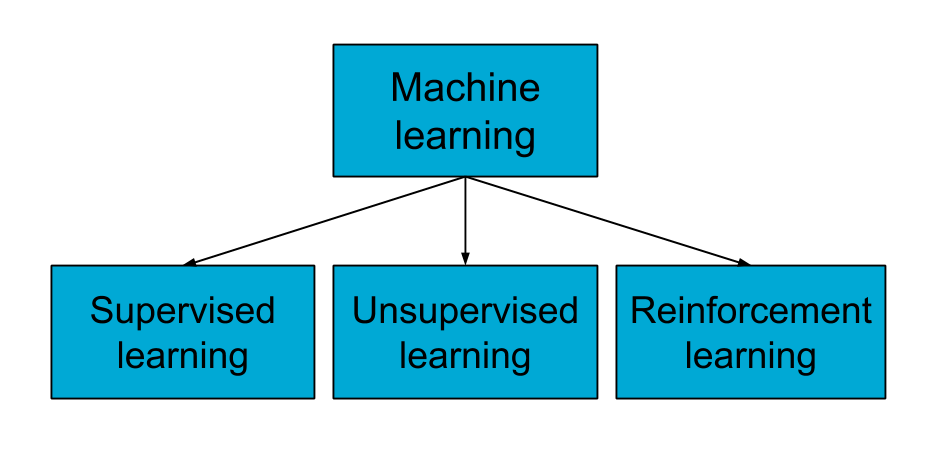
\includegraphics[height=6cm, width=12cm]{figures/supervised_vs_rl.png}
    \caption[size = 9]{The three main categories of machine learning: supervised, unsupervised and reinforcement learning}
    \label{fig:theory:supervised_vs_rl}
\end{figure}


\section{Elements in a reinforcement algorithm}

The agent and the environment with which the agent is interacting is fundamental to any reinforcement learning algorithm. As mentioned in the introduction, an agent is the decision maker that observes a state $s$ and decides what action $a$ to take. An example can be a self-driving vehicle that receives an observation $s$ in the from of input from cameras and sensors placed on the vehicle. The observation $s$ represent the state of the system, and based on that the self-driving car must chose an action $a$. The action might be to turn the wheel to the right which in turn leads to a new observation from the cameras and sensors on the vehicle.

The set of possible actions and states are respectively called the action space $\mathcal{A}$ and state space $\mathcal{S}$. For some reinforcement learning tasks, such as chess, the action space depends on the state $s$. For instance, it is not allowed to castle if an opponents piece is attacking your king. In such cases, the action space $\mathcal{A}(s)$ is given by the state $s$. The action space in an electric power system is dependent on the state, for instance if a power plant or transmission line is out of operation. A central element in the reinforcement algorithm is the reward function $r: \mathcal{S} \times \mathcal{A} \to \mathbb{R}$ that evaluates how "good" action $a$ is in state $s$. For instance, the reward given to the agent in car race can be the the speed of the car so that the agent is incentived to drive fast.

The goal at each time step $t$ is to maximise the rewards in the future. How to formally define the reward maximising criterion depends on the nature of the task. Some tasks, such as playing a video game, are called episodic and have well-defined boundaries for initial and terminal state. On the other hand, the electric power system is a continuous task that never should end if the agent does its job. For continuous tasks, let the discounted return $r^{\gamma}_{t}$ at time $t$ be defined as 


\begin{equation}
   \begin{aligned}\label{eq:theory:discounted_reward}
r^{\gamma}_{t} = r_{t+1} + \gamma r_{t+2} + \gamma^{2} r_{t+3} + ...
= \sum_{k=t}^{\infty} \gamma^{k-t}r_{k+1}
\end{aligned} 
\end{equation}
where $r_{t+1}$ is the reward received after taking action $a_{t}$ in state $s_{t}$,and $\gamma \in [0,1]$ is the discount factor. The goal of the agent at every time step $t$ can be defined to maximise the discounted return $r^{\gamma}_{t}$. The gamma term is a hyper-parameter that can be tuned, and it determines how relevant future rewards are. If $\gamma = 0$, then the agent only considers the immediate reward as relevant. If $\gamma = 1$ then all future rewards count equally to the total future reward $r^{\gamma}_{t}$. Having $\gamma$ less than 1 is also a mathematical convenience that ensures that the discounted return is finite in a continuous task, as long as the rewards are bounded. 

\section{Markov decision process}\label{section:markov_decision_process}

A Markov decision process is a mathematical framework describing sequential decision making and interaction with an environment, where the outcome can be stochastic \cite{Sutton1998}. The environment starts at $t=0$ and is described by an initial state $s_{0} \in \mathcal{S}$. The agent preforms some action $a_{0}\in \mathcal{A}$ and receives a reward $r_{1}\in \mathcal{R} \subseteq \mathbb{R} $ based on how good that action is. The action $a_{0}$ interacts with the environment and gives a new state $s_{1}$. This starts the sequence of states, actions and rewards.


\begin{equation}
   \begin{aligned}\label{eq:theory:trajectory}
s_{0},a_{0},r_{1},s_{1}, a_{1},r_{2},s_{2},...
\end{aligned} 
\end{equation}
The interaction between the agent and environment is visualised in figure \ref{fig:theory:markov_decision_process} as a feedback loop. The loop continues until the environment reaches a terminal state, for instance when the self-driving car reaches its destination or if it crashes. The transitions from start state $s_{0}$ to terminal state $s_{T}$ constitutes an episode in the reinforcement algorithm.  

\begin{figure}[ht!]
    \center
    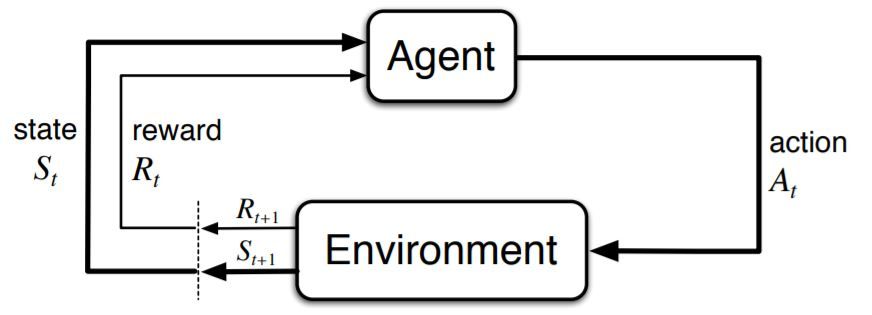
\includegraphics[height=3.5cm, width=10cm]{figures/markov_decision_processs.JPG}
    \caption[size = 9]{Interaction in a Markov decision process. Source: Sutton \cite{Sutton1998}}
    \label{fig:theory:markov_decision_process}
\end{figure}
Formally, a finite Markov decision process $\mathcal{M}$ is a tuple
\begin{equation}
   \begin{aligned}\label{eq:theory:markov_formal}
\mathcal{M} = \langle \mathcal{S},\mathcal{A},\mathcal{P},\mathcal{R},\gamma \rangle
\end{aligned} 
\end{equation}
where $\mathcal{S}$ and $\mathcal{A}$ respectively are finite sets of states and actions, $\mathcal{P}$ is the matrix with state transition probabilities,
$\mathcal{R}$ is a reward function and $\gamma$ is a discount factor \cite{silver_course}. The probability of transitioning to the next state $s_{t+1}$ and receiving $r_{t+1}$ only depends on the previous state $s_{t}$ and action $a_{t}$ in a Markov decision process \cite{Sutton1998}. Formally, a state $s_{t}$ is Markov if and only if 

\begin{equation}
   \begin{aligned}\label{eq:theory:markov_property}
    \mathbb{P}[s_{t+1}|a_{t},\;s_{t}] = \mathbb{P}[s_{t+1}|a_{t},s_{t},\;a_{t-1},s_{t-1},...,a_{0},s_{0}]
\end{aligned} 
\end{equation}
This is called the Markov property of the state \cite{silver_course}. In other words, the history of states and actions leading up to the current state is not relevant for the probability of transition to state $s_{t+1}$. Let the transition function $p: \mathcal{S} \times \mathcal{R} \times \mathcal{S} \times \mathcal{A} \to [0,1]$ be the probability of transitioning from state $s$ to $s'$ and receiving reward $r$ given the action $a$

\begin{equation}
   \begin{aligned}\label{eq:theory:markov_transition}
    p(s',r,s,a) = \mathbb{P}
    [s_{t+1}=s',r_{t+1}=r | s_{t}=s, a_{t} = a]
\end{aligned} 
\end{equation}
If the transition function $p$ in \eqref{eq:theory:markov_transition} is known, it can be used for planning actions in a reinforcement algorithm. 





\section{Value and policy functions}
The reinforcement agent selects an action in a given state through its policy $\pi$. The policy of the agent decides what action to take in a given state by mapping the state space to the action space, $\pi: \mathcal{S} \to \mathcal{A}$. The policy can both be deterministic and stochastic. A deterministic policy maps a given state to the same action every time, while a stochastic policy maps the state to a probability distribution over the action space. For the deterministic case, the policy function $\pi$ is given by


\begin{equation}
   \begin{aligned}\label{eq:theory:policy_function_deterministic}
\pi(s) = a
\end{aligned} 
\end{equation}
where $a$ is the action chosen by the policy. For the stochastic case, it gives the probability of choosing action $a$ in state $s$.


\begin{equation}
   \begin{aligned}\label{eq:theory:policy_function_stochastic}
\pi(a|s) = \mathbb{P}(a|s)
\end{aligned} 
\end{equation}


A central tool in many reinforcement algorithms is to evaluate a certain state before taking an action. The state-value function $V^{\pi}$ is defined as the expected discounted future return in state $s$ under the policy $\pi$.

\begin{equation}
   \begin{aligned}\label{eq:theory:value_function}
V^{\pi}(s) 
&= \mathbb{E}_{\pi}[r^{\gamma}_{t}| s=s_{t}]
\\
&= \mathbb{E}_{\pi}[ r_{t+1} + \gamma r_{t+2} + \gamma^{2} r_{t+3} + ...|s=s_{t}]
\end{aligned} 
\end{equation}

The reason for including "under the policy $\pi$" is that a state is valued differently depending on the policy used. For instance, the start position in chess will be evaluated better under the policy of a chess grand master than under the policy of an amateur, because the grand master has a much higher expected future reward. 



The action-value function $Q^{\pi}$, also called the Q-function, quantifies the expected discounted return given the action $a_{t}$ in state $s_{t}$ and that the policy $\pi$ is followed thereafter. In other words, it can evaluate a specific action in a given state, in contrast to the value function $V$ that only evaluates the state.

\begin{equation}
   \begin{aligned}\label{eq:theory:action_value_function}
Q^{\pi}(s_{t},a_{t}) 
&= \mathbb{E}_{\pi}[r^{\gamma}_{t}|a=a_{t} ,s=s_{t}]
\\
&= \mathbb{E}_{\pi}[ r_{t+1} + \gamma r_{t+2} + \gamma^{2} r_{t+3} + ...|a=a_{t} ,s=s_{t}]
\end{aligned} 
\end{equation}
There is an important recursive relation between the action-value function in two consequent states $s_{t}$ and $s_{t+1}$, known as the Bellman equation. Assuming a deterministic policy $\pi$, we have

\begin{equation}
   \begin{aligned}\label{eq:theory:bellman_equation}
Q^{\pi}(s_{t},a_{t}) 
&= \mathbb{E}[r_{t+1} +\gamma r^{\gamma}_{t+1} |\; s_{t}] \\
& = \mathbb{E}[r_{t+1} +\gamma Q^{\pi}(s_{t+1},\pi(s_{t+1}))|\; s_{t}]
\end{aligned} 
\end{equation}
In other words, the action-value for state $s_{t}$ and action $a_{t}$ is the expected sum of the immediate reward $r_{t}$ and the action-value in the consequent state. The Bellman equation is used in several reinforcement algorithms to guide the estimates of the Q-values closer to the true values.

The action-value function $Q^{\pi}$ and state-value function $V^{\pi}$ are similar to each other and can together be used to measure the advantage of an action $a$. The advantage $A(a,s)$ of action $a$ in state $s$ under policy $\pi$ is defined as 

\begin{equation}
   \begin{aligned}\label{eq:theory:advantage_function}
A(s,a) =  Q^{\pi}(s,a) - V^{\pi}(s)
\end{aligned} 
\end{equation}
If the advantage is positive, it means that it is better to take action $a$ than following the action chosen by the policy in state $s$. Similarly, a negative advantage means that action $a$ is worse than following the action chosen by the policy.

\section{The exploration - exploitation dilemma}
A problem that arises when constructing a reinforcement learning algorithm is how to both be able to exploit a good policy and at the same time explore new policies. If an agent always follows its policy and picks the action it believes is the best, it will never explore new and perhaps better approaches to solve a problem. At the same time, the agent can not simply explore new behaviour all the time, since its goal is to maximise future rewards. Therefore, it must also exploit the behaviour that works. This is called the exploration-exploitation dilemma in reinforcement learning \cite{Sutton1998}. A solution to this problem is two have two different policies. One policy is called the target policy that is to be the optimal solution, while the other is called the behaviour policy and is for exploration of new behaviours \cite{Sutton1998}. A reinforcement learning algorithm using this approach is said to be learning off-policy. On the other hand, on-policy algorithms only learn from the experiences of the agent.

\section{Actor-critic reinforcement learning}
There are two main categories of reinforcement learning algorithms: model-based and model-free reinforcement learning. Model-based algorithm uses the dynamics of the system to plan actions. For instance, the transition function $p$ in equation \eqref{eq:theory:markov_transition}  gives a probability distribution over the next state and reward, which can be used for planning in dynamic programming \cite{silver_course}. The reinforcement algorithm is explicitly using a model of the environment to chose actions. However, for many situations the transition function is unknown, and even if it is known it can be very computationally expensive to use in a reinforcement algorithm.

The second category is called model-free reinforcement learning. As the name suggest, it requires no model or information about the dynamics in the environment. This is very useful in situations where there are no transition function that describes the dynamics in the environment, but experiences can be sampled. Model-free algorithms can be divides into two subcategories: Value-based and policy-based. The categories are visualised in figure \ref{fig:theory:rl_model_modelfree}.


\begin{figure}[ht!]
    \center
    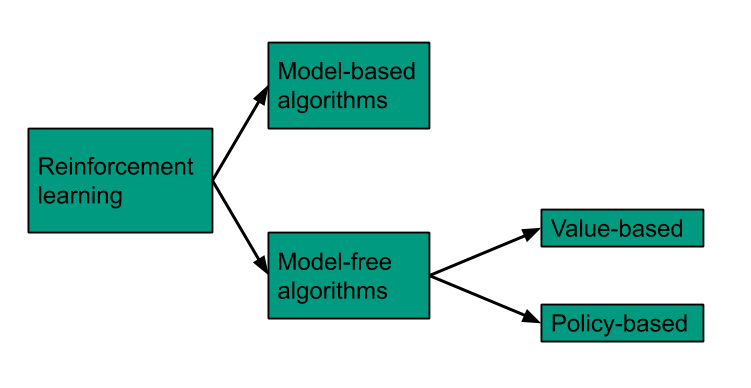
\includegraphics[height=5cm, width=10cm]{figures/rl_model_modelfree.png}
    \caption[size = 9]{Classes of reinforcement algorithms}
    \label{fig:theory:rl_model_modelfree}
\end{figure}


The first subcategory of model-free algorithm is called value-based methods, where the approach is to approximate the action-value function $Q$, and use that to take an action. An example of value-based is Q-learning, SARSA and DQN \cite{Sutton1998}. An advantage of value-based methods is that they can learn off-policy, for instance by learning from the behaviour of experts \cite{value_based_policy_Nachum}. Value-based method are therefore very sample efficient as they do not need to find optimal moves themselves, but can learn from a behaviour that is known to be good. The disadvantage is that value-based methods are not well suited for function approximation, such as neural networks, as they tend to be unstable \cite{Sutton1998}. 

Policy-based methods (also called policy gradient) directly parametrise the policy function $\pi$ without involving the action-value function $Q$ in the decision-making \cite{Sutton1998}. In contrast to value-based methods, they are stable when using function approximation, but very sample inefficient \cite{value_based_policy_Nachum}. In other words, the weakness of value-based methods is the advantage of the policy-based methods, and vice versa. A natural idea is then to combine the two methods into a more robust method. Enter the the actor-critic model. The actor-critic model is a mix of policy-based and value-based reinforcement learning, as illustrated in figure \ref{fig:theory:Actor-critic}. The policy $\pi$ is called the actor, because it chooses the action to take. The action-value function $Q$ is named the critic because it evaluates the action picked by the actor.

\begin{figure}[ht!]
    \center
    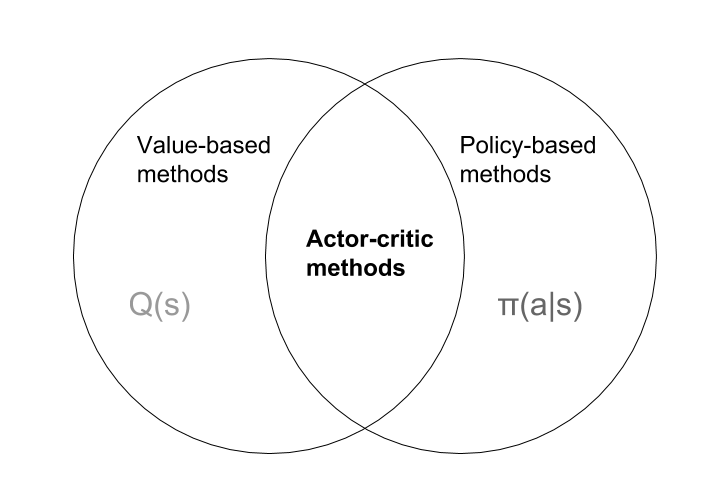
\includegraphics[height=6cm, width=10cm]{figures/Actor-critic.png}
    \caption[size = 9]{Actor-critic in relation to value-based and policy-based methods}
    \label{fig:theory:Actor-critic}
\end{figure}


\section{Deep deterministic policy gradient}
Silver et. al have developed an off-policy reinforcement algorithm called deep deterministic policy gradient (DDPG) \cite{pmlr-v32-silver14}. As the name suggest, the algorithm uses a deterministic approximation of the policy function instead of a stochastic version. The advantage with a deterministic policy is that it does not have to integrate over action space in the search for the best policy. This section will outline the differences between stochastic and deterministic policy function. Both cases share similarities with each other. DDPG models the problem as a Markov decision problem as described in section \ref{section:markov_decision_process}.

The initial state distribution is described by $p_{1}(s_{1})$. There is a reward function $r: \mathcal{S} \times \mathcal{A} \to \mathbb{R}$ and an action value function $Q^{\pi}:\mathcal{S} \times \mathcal{A} \to \mathbb{R}$ that evaluates an action $a$ in state $s$ under the policy $\pi$. The policy interacts with the environment by taking actions and generates a trajectory of states, action and rewards 
\begin{equation}
   \begin{aligned}\label{eq:theory:trajectory2}
h_{1:T} = s_{1},a_{1},r_{1},..., s_{T},a_{T},r_{T}
\end{aligned} 
\end{equation}
The objective function $J(\pi)$ that agent will maximise is the expected discounted return under the policy $\pi$

\begin{equation}
   \begin{aligned}\label{eq:theory:max_discounted_return}
J(\pi)
= \mathbb{E}_{\pi}[r^{\gamma}_{1}]
= \mathbb{E}_{\pi}[ r_{1} + \gamma r_{t+2} + \gamma^{2} r_{t+3} + ...]
\end{aligned} 
\end{equation}

\subsection{Stochastic policy approximation}\label{section:stochastic_policy_approx}
Consider a parametrised stochastic policy $\pi_{\theta}: \mathcal{S}\to \mathcal{P}(\mathcal{A})$ with parameters $\theta^{\pi}$ that maps the state space to a probability distribution over the action space. Let $p(s\to s',t,\pi)$ be the probability of transitioning from state $s$ to $s'$ in $t$ time steps. The discounted state distribution $\rho^{\pi}(s')$ is defined as   

\begin{equation}
   \begin{aligned}\label{eq:theory:discounted_state_distribution}
    \rho^{\pi}(s') = \int_{\mathcal{S}}\sum_{t=1}^{\infty }\gamma^{t-1}p_{1}(s)
    p(s \to s',t,\pi)ds
\end{aligned} 
\end{equation}
The performance objective can then be expressed as an expectation
\begin{equation}
   \begin{aligned}\label{eq:theory:objective_expected_stochastic}
    J(\pi_{\theta}) &= 
    \int_{\mathcal{S}}\rho^{\pi}(s) \int_{\mathcal{A}}\pi_{\theta}(a|s)r(a,s)da ds 
    \\
    &=
    \mathbb{E}_{s\sim \rho^{\pi},a \sim \pi_{\theta}}[r(s,a)]
\end{aligned} 
\end{equation}
 The way the agent learns is by computing the gradient of the objective with respect to the policy parameters $\theta^{\pi}$ and update the weights in that direction. The gradient of the stochastic policy is given by the policy gradient theorem (Sutton \cite{Sutton1998}) in equation \eqref{eq:theory:stochastic_gradient}.

\begin{equation}
   \begin{aligned}\label{eq:theory:stochastic_gradient}
    \nabla_{\theta^{\pi}} J(\pi_{\theta}) &= 
     \int_{\mathcal{S}}\rho^{\pi}(s)
     \int_{\mathcal{A}} \nabla_{\theta^{\pi}} \pi_{\theta}(a|s)Q^{\pi}(a,s)da ds
     \\
     &= \mathbb{E}_{s\sim \rho^{\pi},a \sim \pi_{\theta}}
     [\nabla_{\theta^{\pi}} \log \pi_{\theta}(a|s)Q^{\pi}(a,s) ]
\end{aligned} 
\end{equation}
Equation \eqref{eq:theory:stochastic_gradient} shows that the parameter update for the stochastic policy needs to integrates over the action space, which can be computationally costly.

\subsection{Deterministic policy approximation}
Consider a deterministic policy $\mu_{\theta}: \mathcal{S} \to \mathcal{A}$ with parameters $\theta^{\mu}$. Using the same definitions of discounted state distribution $\rho^{\mu}$ as in equation
\eqref{eq:theory:discounted_state_distribution}, the objective function is given as 

\begin{equation}
   \begin{aligned}\label{eq:theory:objective_expected_deterministic}
    J(\mu_{\theta}) =
    \int_{\mathcal{S}}
    \rho^{\mu}(s)r(s,\mu_{\theta}(s)) ds = \mathbb{E}_{s\sim \rho^{\mu}}[r(s,\mu_{\theta}(s))]
\end{aligned} 
\end{equation}
Silver et al \cite{pmlr-v32-silver14} proved that the deterministic policy gradient is given as 

\begin{equation}
   \begin{aligned}\label{eq:theory:objective_gradient_deterministic}
    \nabla_{\theta^{\mu}}J(\mu_{\theta}) &=
    \int_{\mathcal{S}}
    \rho^{\mu}(s)
    \nabla_{\theta^{\mu}} \mu_{\theta}(s)
    \nabla_{a} Q^{\mu}(s,a)|_{a = \mu_{\theta}(s)}ds 
    \\
    &= \mathbb{E}_{s\sim \rho^{\mu}}
    [    \nabla_{\theta^{\mu}} \mu_{\theta}(s)
    \nabla_{a} Q^{\mu}(s,a)|_{a = \mu_{\theta}(s)}]
\end{aligned} 
\end{equation}
In other words, it is the expectation of the matrix-vector product of the policy Jacobian matrix and the action-value gradient with respect to the actions under policy $\mu_{\theta}$. By convention, the columns of $\nabla_{\theta} \mu_{\theta}$ are the gradient of each action dimension. Silver et al argue that there are a class of function approximators that follow the gradient of the action-value function. Let $\theta^{Q}$ be the parameters of the action-value approximator $Q_{\theta}(s,a)$ such that   

\begin{equation}
   \begin{aligned}\label{eq:theory:action-value_approx}
    Q_{\theta}(s,a) \approx Q^{\mu}(s,a)
\end{aligned} 
\end{equation}
and replace the action-value gradient $\nabla_{a} Q^{\mu}(s,a)$ in equation \eqref{eq:theory:objective_gradient_deterministic} by
the gradient of the approximation $\nabla_{a} Q^{\mu}(s,a,\theta^{Q})$

\subsection{Deterministic off-policy actor-critic}
Deep deterministic policy gradient is an off-policy learning algorithm. An off-policy algorithm has two different policies: a target policy $\mu_{\theta}(s)$ that is to be the final policy, and a stochastic behavioural policy $\beta(s)$ that is used for exploration to find different strategies. In other words, the target policy learns from the experiences of the behavioural policy. The off-policy objective performance in equation \eqref{eq:theory:objective_expected_deterministic} is altered by replacing the reward $r$ with the value function $V^{\mu}$ under the target policy $\mu$ and following the discounted state distribution of the behavioural policy $\rho^{\beta}$.

\begin{equation}
   \begin{aligned}\label{eq:theory:objective_expected_ooff_policy}
    J_{\beta}(\mu_{\theta}) &=
    \int_{\mathcal{S}}
    \rho^{\beta}(s)V^{\mu}(s) ds 
    \\
    &=
    \int_{\mathcal{S}}
    \rho^{\beta}(s)Q^{\mu}(s,\mu_{\theta}(s)) ds
\end{aligned} 
\end{equation}
The gradient of the modified objective is

\begin{equation}
   \begin{aligned}\label{eq:theory:objective_gradient_deterministic_off_policy}
    \nabla_{\theta}J_{\beta}(\mu_{\theta}) &\approx
    \int_{\mathcal{S}}
    \rho^{\beta}(s)
    \nabla_{\theta} \mu_{\theta}(s|a)
    Q^{\mu}(s,a)ds 
    \\
    &= \mathbb{E}_{s\sim \rho^{\beta}}
    [\nabla_{\theta} \mu_{\theta}(s)
    \nabla_{a} Q^{\mu}(s,a)|_{a = \mu_{\theta}(s)}]
\end{aligned} 
\end{equation}

\subsection{Critic loss function}
The bellman equation in \eqref{eq:theory:bellman_equation} can be used in the design of the loss function for the action-value function approximator $Q(s,a|\theta^{Q})$. Let the action-value target $y_{t}$ be defined as 
\begin{equation}
   \begin{aligned}\label{eq:theory:action_value_target_bellman_equation}
y_{t} = r(s_{t},a_{t}) + \gamma Q(s_{t+1},\mu(s_{t+1})|\theta^{Q})
\end{aligned} 
\end{equation}
The action-value loss can be defined as 
\begin{equation}
   \begin{aligned}\label{eq:theory:action_value_loss_bellman_equation}
L(\theta^{Q}) 
&= \mathbb{E}_
{s_{t}\sim\rho^{\beta},a_{t} \sim \beta, r_{t} \sim \mathcal{E}}
[Q(s_{t},a_{t}|\theta^{Q})- y_{t})^{2}]
\end{aligned} 
\end{equation}
Notice that the state and action follows the distribution of the behavioural policy $\beta$. The loss is zero if the action value approximator satisfies the Bellman equation in \eqref{eq:theory:bellman_equation}. Therefore, the action-value approximator is encouraged to satisfy the Bellman equation.

There are however some practical problems with the loss definition in equation \eqref{eq:theory:action_value_target_bellman_equation}. The critic target $y_{t}$ is calculated using $Q(s,\mu(s)|\theta^{Q})$, which after each parameter update of $\theta^{Q}$ may change quickly. Therefore, the critic target can fluctuate rapidly during learning. We are changing our network closer to the target, but the target itself is moving. To avoid this, Lillicrap et al. suggests a soft update of the target weights \cite{DBLP:journals/corr/LillicrapHPHETS15}. This is done by creating a copy of the actor $\mu'$ and critic $Q'$ at the beginning of learning that will serve as the target networks. After each parameter update, the original actor and critic networks $\mu,Q$ are updated as before, while the target weights are soft updated by $\theta' \leftarrow \tau\theta + (1-\tau)\theta'$, where $\tau$ is a small positive number ($\tau  \ll 1$). The target network are more locked in place, and will slowly change during training compared to the original networks. This greatly increase the stability during learning. 


\subsection{Experience replay}
It has been proven difficult to use a naive implementation of the described DDPG algorithm with neural network as function approximators \cite{DBLP:journals/corr/LillicrapHPHETS15}. Learning challenging problems are generally unstable. A problem with the naive approach is that the states and actions explored by the agent during learning are sequential, and by no means uncorrelated. It is best that the samples in a batch used for updating the parameters of a neural network are independent and uncorrelated. A way to get around this problem is by introducing a replay buffer $\mathcal{R}$ where experiences during learning are stored. Specifically, each tuple $(s_{t},a_{t},r_{t},s_{t+1})$ is put into the the replay buffer. When the weights of the functions approximators are updated, a batch of $N$ random transition tuples is drawn from the replay buffer. This avoids the problem with correlated samples in the parameter update and increases the stability of DDPG. In addition, it ensures that the agent does not forget experiences from early in the training. 

\subsection{Algorithm for DDPG}


\begin{algorithm}[H]
\SetAlgoLined
 Randomly initialise critic network $Q(s,a|\theta^{Q})$ and actor $\mu(s|\theta^{\mu})$ with weights $\theta^{Q}$ and $\theta^{\mu}$
 \\
 Initialise target networks $Q'$ and $\mu'$ with weights $\theta^{Q'} \leftarrow \theta^{Q}$ and $\theta^{\mu'} \leftarrow \theta^{\mu}$ 
 \\
 Initialise replay buffer $\mathcal{R}$
 \\
 \For{episode 1:M}{
  Initialise random process $\mathcal{N}$\\
  Receive initial state $s_{1}$
  
  \For{t 1:T}{
   Select $a_{t} = \mu(s_{t}|\theta^{Q}) + \mathcal{N}_{t}$
   \\
   Execute $a_{t}$ and observe reward $r_{t}$ and new state $s_{t+1}$
   \\
   Store transition $(s_{t},a_{t},r_{t},s_{t+1})$  in replay buffer $\mathcal{R}$
   \\
   Sample random minibatch of N transitions from the replay buffer
   \\
   Set critic target $y_{i} = r(s_{i},a_{i}) + \gamma Q'(s_{i+1},\mu'(s_{i+1})|\theta^{Q'})$
   \\
   Update critic by
   \begin{equation}
   \begin{aligned}\label{eq:theory:DDPG_critic_update}
   L =\frac{1}{N}\sum_{i=1}^{N}Q(s_{t},a_{t}|\theta^{Q})- y_{t})^{2}
\end{aligned} 
\end{equation}
Update actor policy by
\begin{equation}
   \begin{aligned}\label{eq:theory:DDPG_actor_update}
   \nabla_{\theta^{\mu}}J \approx
   \frac{1}{N}\sum_{i=1}^{N}
   \nabla_{a} Q(s,a|\theta^{Q})|_{s=s_{i},a = \mu(s_{i})}
   \nabla_{\theta^{\mu}} \mu(s|\theta^{\mu})|_{s=s_{i}}
\end{aligned} 
\end{equation}
Soft update the target weights

\begin{equation}
   \begin{aligned}\label{eq:theory:DDPG_target_soft_update}
     &\theta^{Q'} \leftarrow \tau\theta^{Q} + (1-\tau)\theta^{Q'}
     \\
     &\theta^{\mu'} \leftarrow \tau\theta^{\mu} + (1-\tau)\theta^{\mu'}
    \end{aligned} 
\end{equation}
   
   }{
   
  }
 }
 \caption{Deep deterministic policy gradient, as described by Lillicrap et al.\cite{DBLP:journals/corr/LillicrapHPHETS15}}
\end{algorithm}

\section{Hindsigth Experience Replay}
TODO: Remove HER?
\subsection{Challenging reward engineering}\label{theory:challenging_reward_shaping}

Designing the reward for a reinforcement agent is often a challenging and time-consuming task. For an algorithm attempting to play a game it is usually not a problem, since the reward could simply be the score in the game, or a positive reward every time the agent wins an episode. However, for other tasks there will often be a need for a lot of handcrafted rewards that require domain-specific knowledge. This section will present an example of this challenge in an electric power system.

\begin{figure}[ht!]
    \center
    \subimport{../}{circuits/two_bus.tex}
    \caption[size = 9]
    {Simple two bus system connected by a line. \textit{P} and \textit{Q} are the active and reactive power flow, \textit{R} and \textit{X} is the resistance and reactance of the line, \textit{U} is the voltage and \textit{I} is the current flowing}    \label{fig:theory:two_bus_reinforcement}
\end{figure}





Consider the two-bus system shown in figure \ref{fig:theory:two_bus_reinforcement}. The bus at the left represent a power plant that produces electric power $S_{1} = P_{1} + jQ_{1}$. The power flows through the transmission line and with some losses and arrives at bus 2 with apparent power $S_{2} = P_{2} + jQ_{2}$. An agent using the deep deterministic policy gradient (DDPG) algorithm was given a simple load balancing task on the power network. The agent controls the active power production $P_{1}$ at bus 1, and has to tune it so that bus 2 receives the desired active load $P_{2}$. For simplicity, the demanded load at bus 2 is constant at 1.3 MW. The voltages magnitudes at each bus is locked to 1 p.u, while the reactive power injections and voltage angle can vary. The reward $r_{t}$ is defined as the negative of the absolute deviation between the received and desired load at bus 2. The idea is that the agent should be encouraged to move closer to the desired load. For simplicity, the initial state, represented as the voltage magnitude, voltage angle the apparent power at each bus, was always the same. The task should therefore be very manageable for the agent because it only has to learn one simple behaviour. After training it converged and received rewards close to 0, indicating that bus 2 got the desired load. The problem was that the agent produced over 10 times as much active power as bus 2 wanted. Where did the rest go? It was lost in the line. In other words, the system had under 10 \% efficiency. Figure \ref{fig:theory:two_bus_failing} shows what was happening. A line can not transfer an arbitrary amount of active power due to the power flow equations. As a result, there will be two different production points for $P_{1}$ that gives the load the desired amount of active power. However, the production point around 12 MW is obviously not desired, as the system efficiency is below 10 \%. However, one cannot blame the agent for finding this point, and sticking with it. It has no incentive to change its behaviour when the reward is defined as it is. A natural solution would be to include a term in the reward that punishes loss in the line. This can be done, and the agent would probably find the right power production level. This illustrates the challenges with manual reward shaping. 

\begin{figure}[ht!]
    \center
    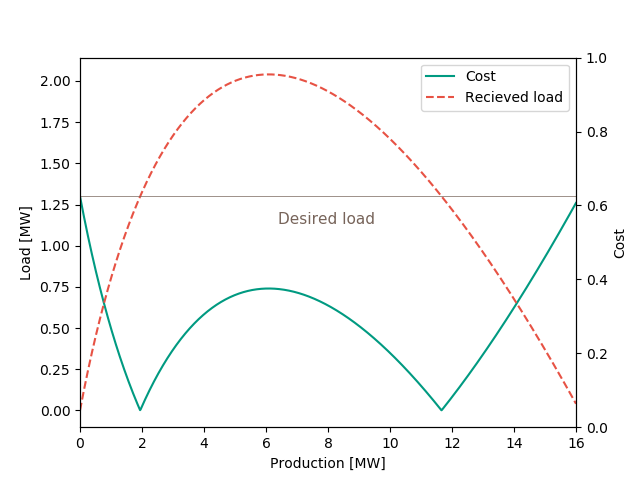
\includegraphics[height=7.5cm, width=10cm]{figures/twobus_load_balance.png}
    \caption[size = 9]{Received load as a function of production of the two-bus system in figure \ref{fig:theory:two_bus_reinforcement}, and cost given to the agent}
    \label{fig:theory:two_bus_failing}
\end{figure}


\subsection{Intuition for Hindsight Experience Replay}
Section \ref{theory:challenging_reward_shaping}  illustrates the challenges with reward shaping and the need for domain-expertise. Hindsight Experience Replay (HER) is an approach that avoids the need for custom made rewards for any off-policy reinforcement learning algorithm, such as DDPG \cite{DBLP:journals/corr/Andrychowicz_HER}. HER modifies Universal Value Function Approximators (UVFA), a method that feeds the agent with a goal $g$ that represent the state at which we want to be. By doing so, the agent does not only generalise to arbitrary states, but also arbitrary goals \cite{schaul15_goal_states}. This is ideal for reinforcement learning in an electric power system. The
supply and demand for electric power are varying every hour in the Norwegian power system, and it is therefore essential that the agent can learn to generalise its behaviour to new and unseen demand situation. 

The sparse reward can simply be -1 at every time step when the goal $g$ is not reached, and 0 if the actual state is within some threshold from the goal. However, this approach is not well suited for a large state space, since the agent never will encounter a non-negative reward \cite{DBLP:journals/corr/Andrychowicz_HER}. The reward is simply too sparse and non-informative. The novelty in HER is to change the goal state for certain transitions in the replay buffer to a state that actually was visited by the agent. As a result, the agent will experience some positive rewards during learning. Although a visited state was far from the desired goal, it still can learn from it because the transitions leading to an unwanted actual state tells the agent something about how to reach that very state. 

DDPG stores the transitions experienced during learning $(s_{t},a_{t},r_{t},s_{t+1})$ in a replay buffer $\mathcal{R}$. This transition tuple is now extended to include the goal state $g$. In other words, a transition in the replay buffer takes the form $(s_{t},a_{t},r_{t},g,s_{t+1})$ where $g$ is the goal shared between all time steps in an episode. The details of HER will be described in the following sections.

\subsection{Algorithm}

The policy and action-value functions are given a goal $g$ in addition to the state $s$ and action $a$. Let $\mathcal{G}, \mathcal{S}, \mathcal{A}$ be the space of all goals, states and actions respectively. 

\begin{equation}
   \begin{aligned}
   \label{eq:theory:her_function_with_goal}
    &Q: \mathcal{S} \times \mathcal{A} \times \mathcal{G} \to \mathbb{R}
    \\
    &\pi: \mathcal{S} \times \mathcal{G} \to \mathcal{A}
    \\
    &r: \mathcal{S} \times \mathcal{A} \times \mathcal{G} \to \mathbb{R}
    \end{aligned} 
\end{equation}
where $Q$ is the action-value function, $\pi$ is the policy function and $r$ is the reward function. The change in all these function is the inclusion of the goal. For each episode there will be a goal state that the policy and action-value takes in as input for all time steps. For each goal state $g$ there will be an associated predicate function $f_{g}: \mathcal{S} \to \{0,1\}$ and the task for the agent is to find a preform an action such that the next states maps to 1. If we for instance let $\mathcal{G} = \mathcal{S}$, the predicate could be $f_{g}(s) = [s=g]$. In other words, a given state maps to 1 if it is the desired goal. The sparse reward to the agent can then be formulated as $r_{g}(s,a) = -[f_{g}(s)=0]$. For continuous states and goals it would be more convenient to have a threshold $\epsilon$ such as $f_{g}(s) = [|s-g| < \epsilon]$ The goal vector could in an electric power system be the desired loads







\end{document}

